
\vspace{1.5cm}


En la figura~\figref{fig:fig_p15_voltage_vs_current} se muestra la variación de la tensión de salida en función de la corriente de salida, se distinguen claramente y están marcadas, las regiones de regulación de tensión (la tensión nominal esperada es de $2 \si[per-mode=symbol]{\volt}$) y corriente (la corriente esperada es de $2 \si[per-mode=symbol]{\ampere}$).




\vfill

\clearpage

\begin{figure}[H] %htb
\begin{center}
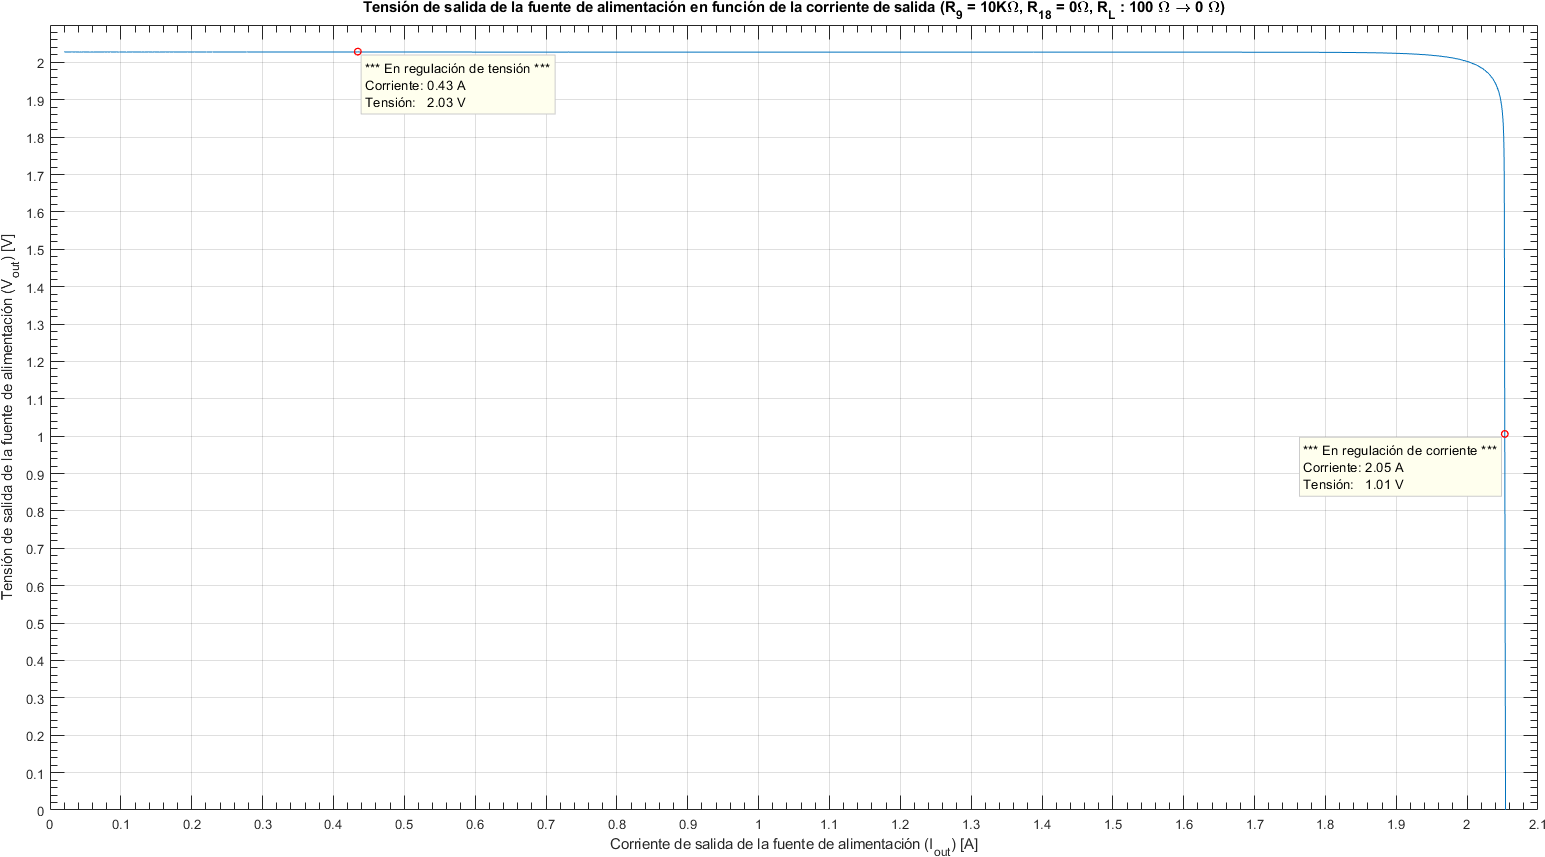
\includegraphics[width=1.2 \textwidth, angle=90]{./img/preguntas/p15.png}
\caption{\label{fig:fig_p15_voltage_vs_current}\footnotesize{Tensión de salida en función de la corriente de salida para $R_{L}$ variando entre $100 \si[per-mode=symbol]{\ohm} y 0 \si[per-mode=symbol]{\ohm}$.}}
\end{center}
\end{figure}



\clearpage
